\documentclass[UTF8]{ctexart}
\usepackage{ctex}
\usepackage{geometry}
\usepackage{enumitem}
\usepackage{indentfirst}
\usepackage{color}
\usepackage{fancyhdr}
\usepackage{amsmath}
\usepackage{graphicx}
\usepackage{amssymb}
\usepackage{tikz}
\usepackage{cases}
\usepackage{array}
\usepackage{pgfplots}
\usepackage{tkz-euclide}
\usepackage{mathrsfs}
% 设置纸张和页边距——A4
\geometry{papersize={21cm,29.7cm}}
\geometry{left=3.18cm,right=3.18cm,top=2.54cm,bottom=2.54cm}

% 一级标题靠左
\CTEXsetup[format={\Large\bfseries}]{section}

% 去除页眉
\pagestyle{plain}

%设置段间距
\addtolength{\parskip}{.4em}
%%设置行间距
%\usepackage{setspace}
%\setstretch{2.5}

% 开始文档内容
\begin{document}

\title{信号与系统课程笔记:Lecture 21:H(s)}
\author{授课教师:秦雨潇 \\
        笔记记录:曹时成}
\date{2023 年 11 月 22 日(第十二周,周三)}
\maketitle

\section{复习}
我们的系统可以(抽象)表达为:\par
例:$y''(t) + ay'(t) + by(t) = cf(t) \equiv f(t) \rightarrow \boxed{\text{$h(t)$}} \rightarrow y(t)$ \par
解题“套路”:$s^2Y(s)-sy(0_-)-y'(0_-)+a(sY(s)-y(0_-))+bY(s)=cF(s)$ \par
化简合并:$(s^2+as+b)Y(s)-[(s+a)y(0_-)+y'(0_-) ]=cF(s) $ \par
得:$Y(s)=\frac{(s+a)y(0_-)+y'(0_-)}{s^2+as+b} +\frac{c}{s^2+as+b}F(s) $ \par
\qquad $\Longrightarrow y(t)=\mathscr{L}^{-1}\{ Y(s)\} $  \par
\section{H(s)}
\subsection{H(s)是什么?}
H(s):系统函数/转移函数(Transfer Function)  \par
对于:$H(s)\longleftrightarrow H(w)\longleftrightarrow h(t)$ \par 
H(s): s域响应; \par 
H(w):频域响应; \par 
h(t):脉冲响应函数(IRF)。 \par 

\subsection{H(s)$\longrightarrow $如何求解?从“工程角度”求解逆变换}
从H(s)求解h(t): \par 
\qquad $H(s)=\frac{b_ms^m+b_{m-1}s^{m-1}+\cdots +b_1s+b_0}{s^n+a_{n-1}s^{n-1}++a_{n-2}s^{n-2}+\cdots +a_1s+a_0} $\par 
(1)当m<n时:\par
\qquad $H(s)=\frac{k_1}{s-p_1}+ \frac{k_2}{s-p_2}+ \cdots +\frac{k_n}{s-p_n}$\par
于是$p_i$的值已知,求解 $k_i$:\par
情况1,分母无重根的情况下求解 $k_i$:\par
\qquad $H(s)(s-p_i)\mid _{s=p_i}=k_i$\par
情况2,分母有重根的情况下求解 $k_i$:\par
\qquad 例:$H(s)=\frac{k_{11}}{(s-p_1)^3}+\frac{k_{12}}{(s-p_1)^2}+\frac{k_{13}}{(s-p_1)}+\frac{k_2}{(s-p_2)} \equiv \frac{\text{略}}{(s-p_1)^3(s-p_2)}$\par
于是:\par
\qquad $H(s)(s-p_i)^3\mid _{s=p_1}=k_{11}$\par
\qquad $\frac{d[H(s)(s-p_i)^3 ] }{ds} \mid _{s=p_1}=k_{12}$\par
\qquad \qquad $\vdots $\par
(2)当m>n时:\par
H(s)化简为$a_0+$(m<n的部分)\par
例如:$H(s)=\frac{s+3}{s+2}=1+\frac{1}{s+2} $\par
例题1:$H(s)=\frac{s-2}{s(s+1)^3}=\frac{k_{11}}{(s+1)^3}+\frac{k_{12}}{(s+1)^2} +\frac{k_{13}}{(s+1)}+\frac{k_2}{(s+1)} $\par
解:\par
\qquad $k_{11}=H(s)(s-p_1)^3\mid _{s=-1}=(\frac{s-2}{s} )\mid _{s=-1}=3$\par
\qquad $k_{12}=(\frac{s-2}{s} )'\mid _{s=-1}=2$\par
\qquad $k_{13}=(\frac{s-2}{s} )''\mid _{s=-1}=4$\par
\qquad $k_{2}=H(s)(s-p_2)\mid _{s=0}=(\frac{s-2}{(s+1)^3} )\mid _{s=0}=-2$\par
于是:$h(t)=[(\frac{3}{2}t^2+2t+4 )e^{-t}-2 ]u(t) $\par
\textbf{作业:书上例5-8至例5-15} \par

\subsection{如何理解H(s)?$\equiv $ 零极图 }
H(s)可以写成如下形式:\par
\qquad $H(s)=\frac{k(s-z_1)(s-z_2)\cdots (s-z_m)}{(s-p_1)(s-p_2)\cdots (s-p_n)} $\par  
零极图:$p_i$是极点,$z_i$是零点 \par  
\begin{figure}[h]
    \centering         %使图片居中放置
    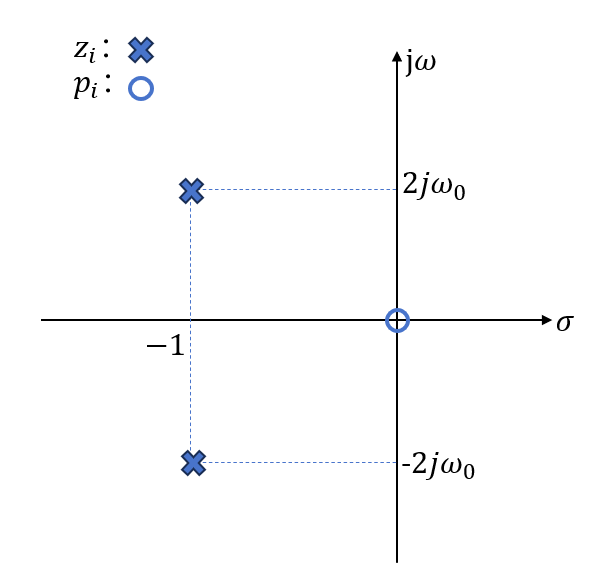
\includegraphics[scale=0.40]{1.png}
    \caption{零极图}
\end{figure}
\textbf{零极图的作用以及和H(s)的关系?} \par
(1)只看零极图,就可以写出H(s)\par
$H(s)=\frac{ks}{(s-(-1+2j))(s-(-1-2j))} =\frac{ks}{(s^2+2s+5)}$ \par
其中H(s)中的k作为一个常数项,在零极图中并不能体现出来。\par
\begin{figure}[h]
    \centering         %使图片居中放置
    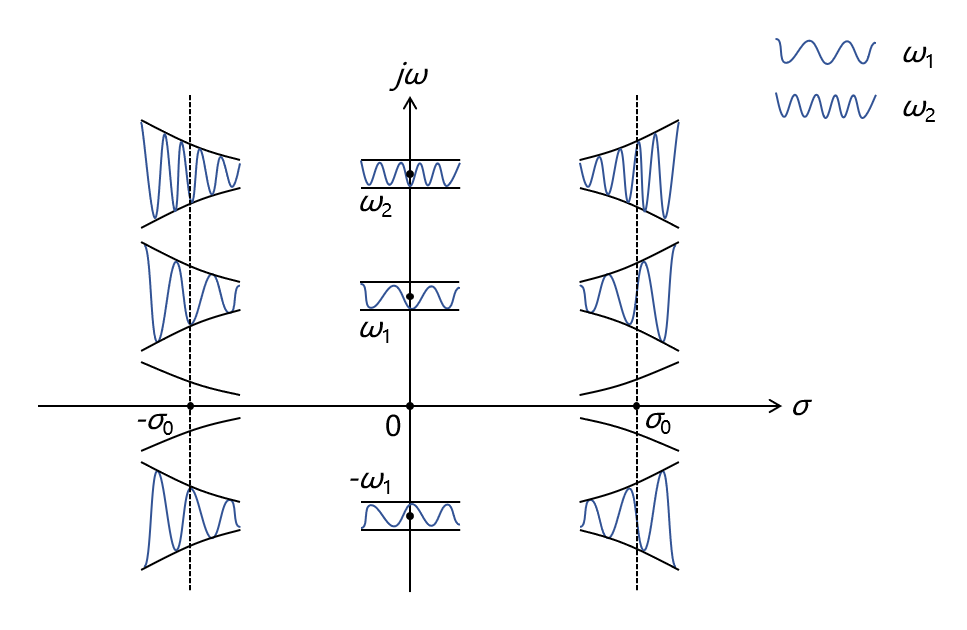
\includegraphics[scale=0.45]{2.png}
    \caption{零极图上的谐波函数}
\end{figure}
当$\delta=0$时,拉普拉斯变换为傅里叶变换 \par
\begin{figure}[h]
    \centering         %使图片居中放置
    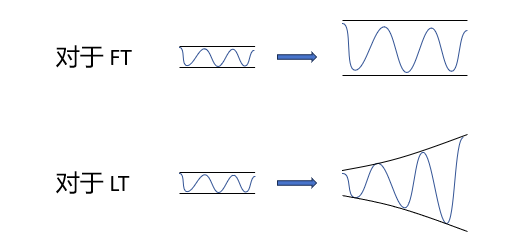
\includegraphics[scale=0.45]{3.png}
\end{figure}
(2)零极图可以直接看出系统的“性质”(“频率响应”)\par
(3)收敛域\par
$\lim_{t \to +\infty}f(t)e^{-\delta t}=0\Longleftrightarrow   $系统稳定\par
收敛域:$\delta_c<0$,$F(w)=F(s)\vert _{\delta=0}$\par
系统稳定$\Longleftrightarrow $极点都在jw轴以左。\par
\end{document}